\documentclass[numbers=noenddot,12pt,a4paper]{scrartcl}
\usepackage[greek,ngerman]{babel}
\usepackage[T1]{fontenc}
\usepackage[utf8]{inputenc}
\usepackage{fullpage}
\usepackage{libertine}
\usepackage{ziffer}
\usepackage{graphicx}
\usepackage{units}
%\usepackage{wasysym}
\usepackage{amsmath}
\usepackage{amssymb}
\usepackage{wrapfig}
\usepackage{esint}
\usepackage{float}
\usepackage{wrapfig}
\usepackage[font=small]{caption}
\usepackage{subcaption}

\renewcommand{\thefigure}{Abb. \arabic{figure}}

\captionsetup[wrapfigure]{name=}
\captionsetup[figure]{name=}
\newcommand{\degree}{^\circ}
\newcommand{\diff}{\textnormal{d}}
\newcommand{\tenpo}[1]{\cdot 10^{#1}}
\newcommand{\greek}[1]{\greektext#1\latintext}
\newcommand{\ix}[1]{_\text{#1}}
\newcommand{\imag}{\mathbf{i}}

\title{Protokoll: Operationsverstärker I}
\author{Tom Kranz, Philipp Hacker}
\date{\today}

\begin{document}
%\setcounter{page}{2}
%\setcounter{section}{1}
\maketitle
\vspace*{\fill}
\tableofcontents
\vfill
\newpage
\section{Vorbereitung}
\subsection{Vorbereitungsaufgabe 1}
Die Kenngrößen eines Operationsverstärkers sind die Differenzverstärkung $A\ix{D}(w)$ (i.A. von der Frequenz abhängig), die Differenzeingangsspannung $U\ix{D}=U_+-U_-$ (siehe \ref{img:ersatzopv}) sowie die Eingangs- bzw. Ausgangswiderstände  $r\ix{G}$ und  $r\ix{a}$. Dabei gilt $A\ix{D}(w)\propto\frac{U\ix{a}}{U\ix{D}}$. Ein idealer Operationsverstärker ist durch eine unendlich große, frequenzunabhängige Differenzverstärkung gekennzeichnet. Für ihn werden die Eingangswiderstände als unendlich groß und der Ausgangswiderstand als 0 angenommen (siehe Schaltskizze \ref{img:ersatzopv}). Somit folgt, dass der ideale OPV eine unendlich große Bandbreite  besitzt und die ansteuernde Spannungsquelle nicht belastet wird. Wiederum kann der Ausgang des OPV schwach belastet werden, ohne das $U\ix{a}$ zusammenbricht. Für reale Operationsverstärker gelten diese Annahmen jedoch nur in erster Näherung: $A\ix{D}(w)$ ist im Allgemeinen stark frequenzabhängig (siehe Bodediagramm \ref{img:bode}; $A\ix{D}\in\left[10^4\dots10^7\right]$) und wird für Frequenzen größer der Transitfrequenz $f\ix{t}$ sogar $<1$. Die Gleichtaktwiderstände $r\ix{G}\in\left[10^9\Omega\dots10^{15}\Omega\right]$, der Ausgangswiderstand $r\ix{a}\in\left[30\Omega\dots1000\Omega\right]$ und der Differenzeingangswiderstand $r\ix{D}\in\left[10^6\Omega\dots10^{12}\Omega\right]$ weichen mehr oder weniger stark von den Idealisierungen ab, was die Belastung der ansteuernden/angesteuerten Systeme sowie die Leistung des OPV empfindlich beeinflusst.
\begin{figure}[H]
\centering
\begin{subfigure}[b]{0.48\textwidth}
\centering
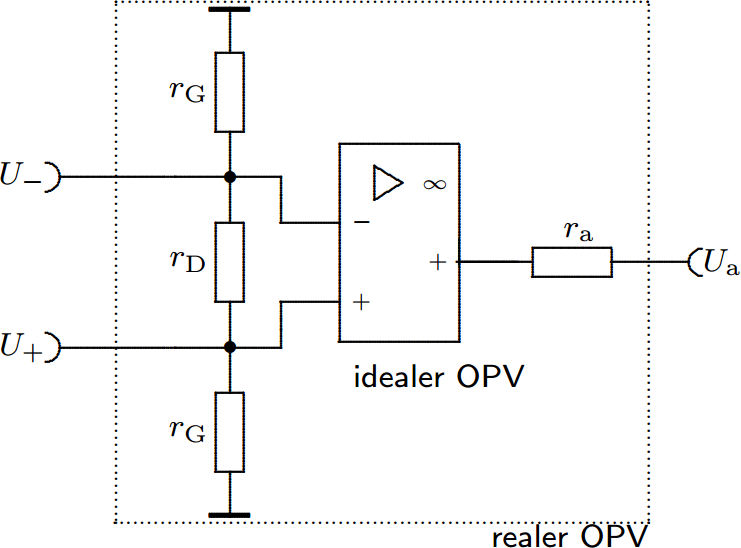
\includegraphics[width=\textwidth]{realopv.png}
\caption{Ersatzschaltbild \\ \vspace{2.6em}} \label{img:ersatzopv}
\end{subfigure}
\begin{subfigure}[b]{0.48\textwidth}
\centering
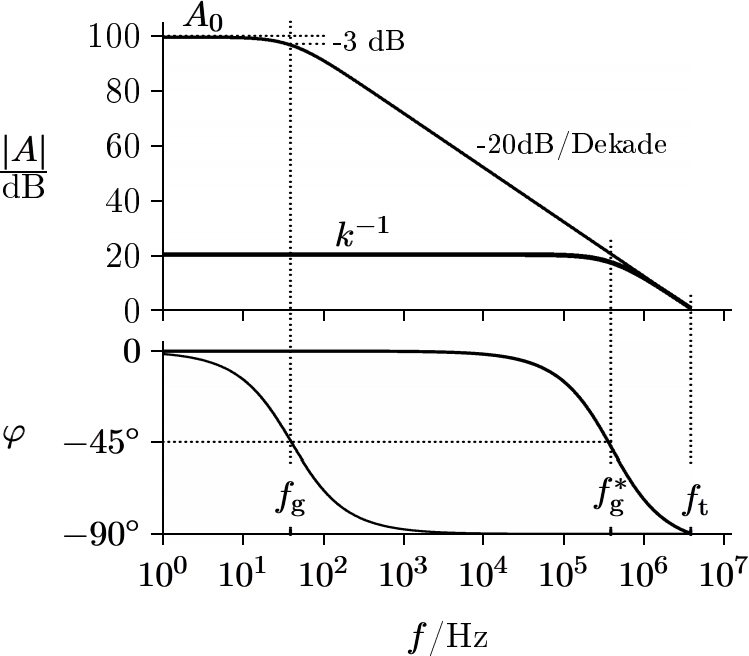
\includegraphics[width=\textwidth]{bodedia.png}
\caption{doppellogarithmisches Bode- und Phasendiagramm mit Vergleich zur Gegenkopplung ($k^{-1}=10$)} \label{img:bode}
\end{subfigure}
\caption{realer Operationsverstärker}
\end{figure}
\subsection{Vorbereitungsaufgabe 2}
\begin{align*}
A(w)=\frac{\frac{1}{k}}{1+\imag\cdot\frac{w}{k\cdot A_0\cdot w_g}}=&\frac{A\ix{D}}{1+k\cdot A\ix{D}} \\
k\approx\frac{R_1}{R_1+R_2} \; ; \; z=\frac{w}{w_g} \rightarrow A\ix{D}(w)=&\frac{A_0}{1+\imag\cdot z} \\
\rightarrow A(w)=&\frac{\frac{1}{k}}{1+\imag\cdot \frac{z}{k\cdot A_0}}
\end{align*}
\subsection{Vorbereitungsaufgabe 3}
\begin{figure}[H]
\vspace{5cm}
\caption{Ersatzschaltbild der Elektrometer-Gegenkopplung} \label{img:ersatzskizze}
\end{figure}
\begin{align*}
\frac{\Delta U\ix{a}}{\Delta U\ix{D}}=A\ix{D} \hspace{0.5cm}&\hspace{0.5cm} \frac{\Delta U\ix{e}}{k}=\Delta U\ix{a} \\
\frac{\Delta U\ix{D}}{r\ix{D}}=\frac{\Delta U\ix{e}}{k\cdot A\ix{D}\cdot r\ix{D}} \hspace{1cm} \Delta I\ix{D}=&\frac{\Delta U\ix{e}}{r\ix{G}} \hspace{1cm} \Delta I\ix{G}=\frac{\Delta U\ix{e}}{r\ix{G}} \\
\Delta I\ix{e}=\Delta I\ix{G}+\Delta I\ix{D}&=\Delta U\ix{e}\cdot\left(\frac{1}{k\cdot A\ix{D}\cdot r\ix{D}}+\frac{1}{r\ix{G}}\right) \\
\rightarrow r\ix{e}=\frac{\Delta U\ix{e}}{\Delta I\ix{e}}=&\left(\frac{1}{k\cdot A\ix{D}\cdot r\ix{D}}+\frac{1}{r\ix{G}}\right) \\
\Delta \widetilde{U}\ix{a}=A\ix{D}\cdot U\ix{D} \hspace{1cm} \Delta U\ix{a}=&\Delta\widetilde{U}\ix{a}-r\ix{a}\cdot\Delta I\ix{a} \hspace{1cm} \Delta U\ix{D}=-k\cdot\Delta U\ix{a} \\
\widetilde{r}\ix{a}=-\frac{\Delta U\ix{a}}{\Delta J\ix{a}}=&-\frac{k\cdot A\ix{D}\cdot\Delta U\ix{a}+r\ix{a}\cdot\Delta I\ix{a}}{\Delta I\ix{a}} \\ \rightarrow \widetilde{r}\ix{a}=&\frac{r\ix{a}}{1+k\cdot A\ix{D}}
\end{align*}
\subsection{Vorbereitungsaufgabe 4}
\begin{align*}
r\ix{i}=\frac{\Delta U\ix{i}}{\Delta I\ix{i}}\approx R\ix{i} \hspace{0.5cm} & \hspace{0.5cm} \widetilde{r}\ix{a}=\frac{\Delta U\ix{a}}{\Delta I\ix{a}}\approx\frac{r\ix{a}}{1+k\cdot A\ix{D}} \\
\rightarrow k=&\left.\frac{U_-}{U\ix{a}}\right|_{U\ix{e}=0}
\end{align*}
\subsection{Vorbereitungsaufgabe 5}
\begin{figure}[H]
\centering
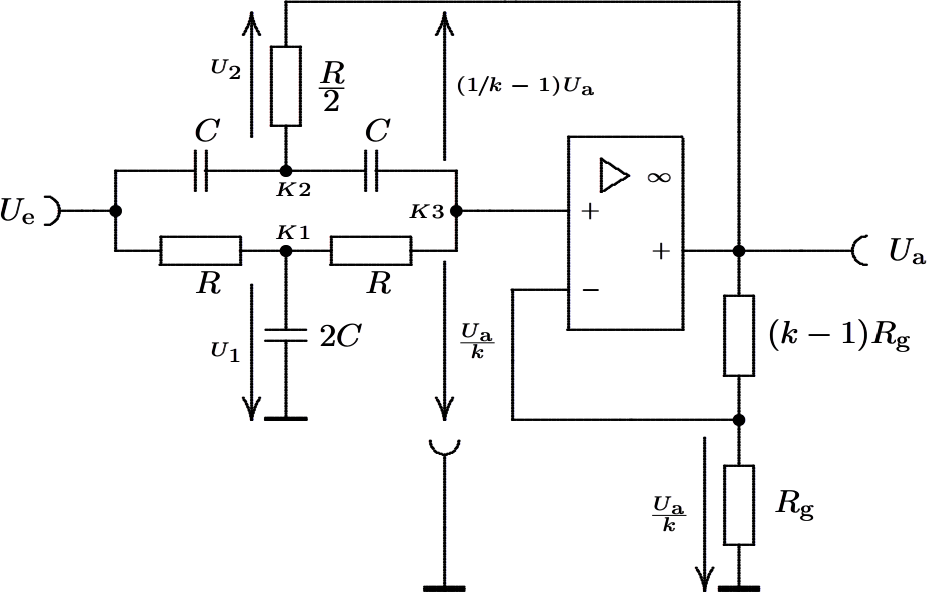
\includegraphics[width=0.6\textwidth]{bandsperre.png}
\caption{Schaltbild der Bandsperre} \label{img:skizze5}
\end{figure}
\begin{align*}
\textbf{K1: } U_1=\frac{k\cdot U\ix{e}+U\ix{a}}{2\cdot k\cdot\left(1+P\right)} \hspace{0.5cm}&\hspace{0.5cm} \textbf{K2: } U_2=\frac{\left(k\cdot U\ix{e}+\left(1-2\cdot k\right)\cdot U\ix{a}\right)\cdot P}{2\cdot k\left(1+P\right)} \\
\textbf{K3: }\left(\left(1-k\right)\cdot P+1\right)\cdot U\ix{a}&=\frac{k\cdot U\ix{e}+U\ix{a}}{2\cdot \left(1+P\right)}+\frac{\left(k\cdot U\ix{e}+\left(1-2\cdot k\right)\cdot U\ix{a}\right)\cdot P^2}{2\cdot\left(1+P\right)} \\
A=\frac{U\ix{a}}{U\ix{e}} \rightarrow & \left(\left(1-k\right)\cdot P+1\right)\cdot A=\frac{k+ A+\left(k+\left(1-2\cdot k\right) \cdot A\right)\cdot P^2}{2\cdot\left(1+P\right)} \\
\rightarrow A=&\frac{k\cdot \left(1+P^2\right)}{1+2\cdot \left(2-k\right)\cdot P+P^2}
\end{align*}
\subsection{Schaltskizzen}
\begin{figure}[H]
\centering
\begin{subfigure}[b]{0.48\textwidth}
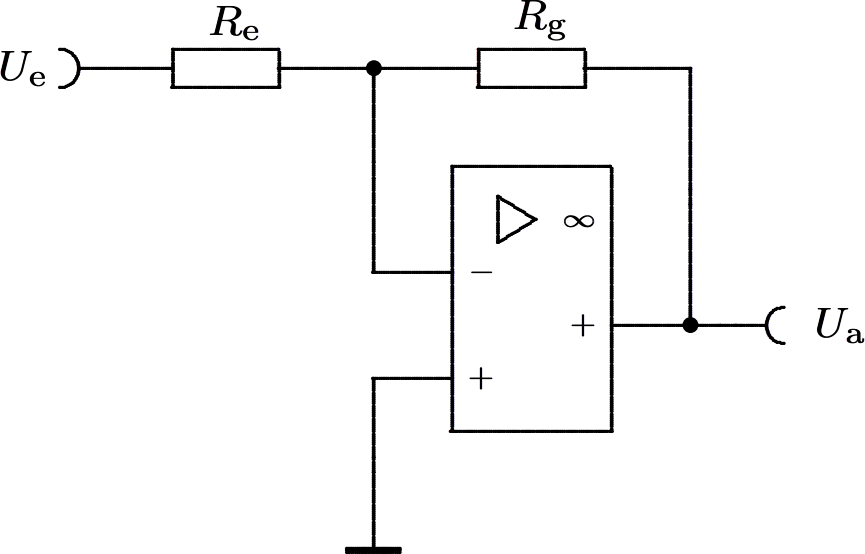
\includegraphics[width=\textwidth]{invertierender.png}
\caption{invertierender Verstärker} \label{img:invert}
\end{subfigure}
\begin{subfigure}[b]{0.48\textwidth}
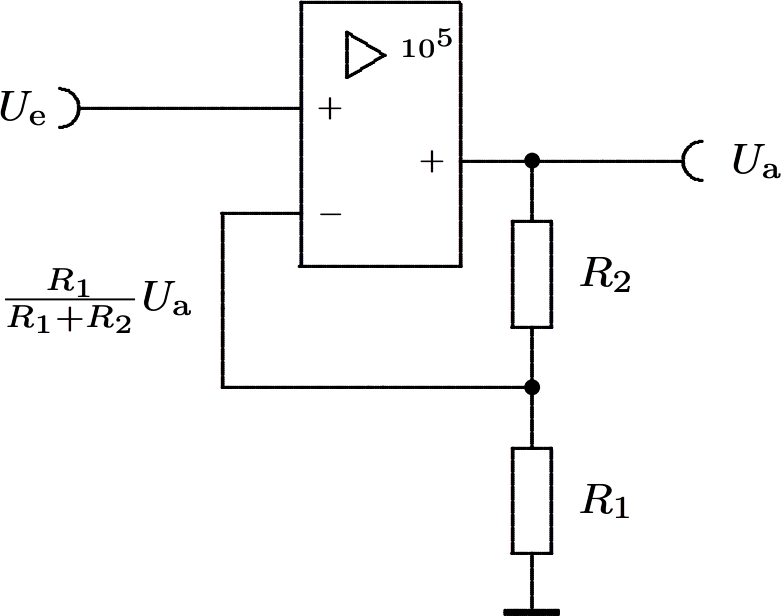
\includegraphics[width=\textwidth]{nichtinvert.png}
\caption{nicht-invertierender Verstärker} \label{img:ninvert}
\end{subfigure}
\end{figure}
\begin{figure}[H]
\centering
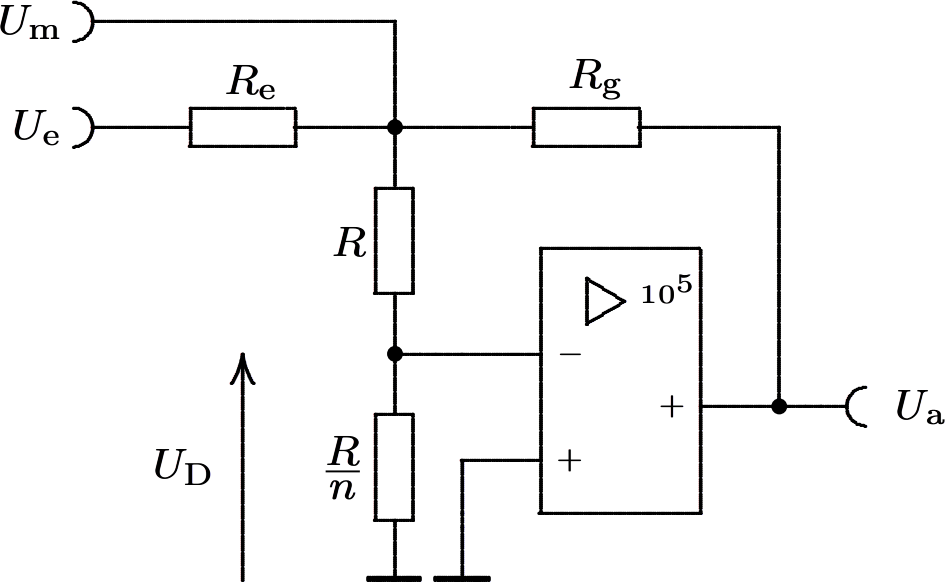
\includegraphics[width=0.6\textwidth]{messungssch.png}
\caption{Schaltung zur Messung der Differenzverstärkung} \label{img:messung}
\end{figure}
\begin{figure}[H]
\begin{subfigure}[b]{0.48\textwidth}
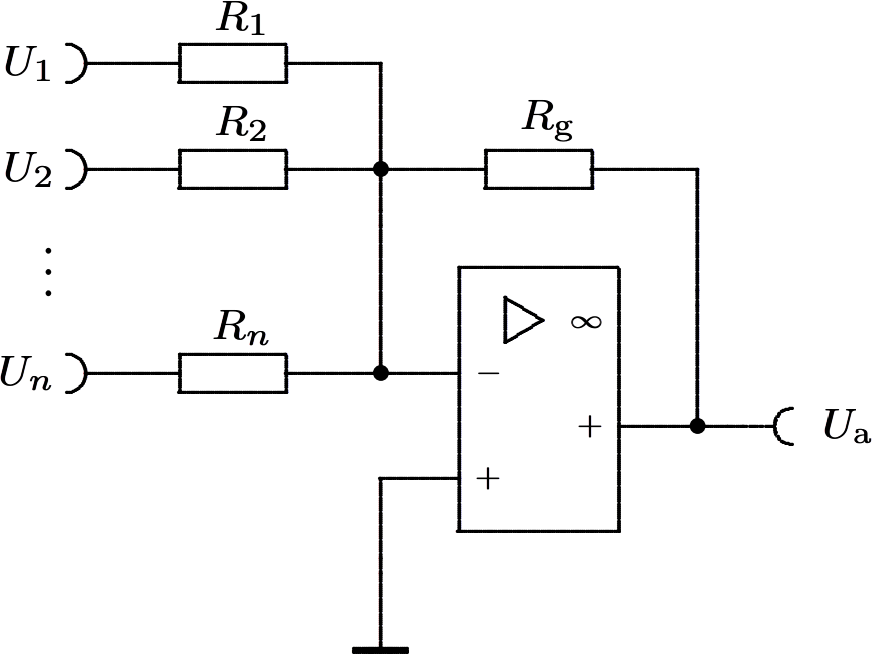
\includegraphics[width=\textwidth]{summation.png}
\caption{invertierender Summationsverstärker} \label{img:summ}
\end{subfigure}
\begin{subfigure}[b]{0.48\textwidth}
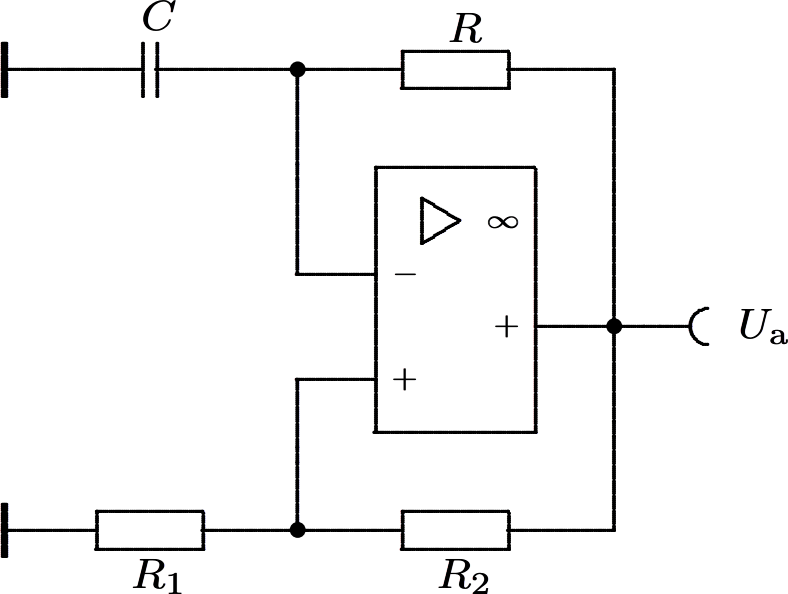
\includegraphics[width=\textwidth]{multivib.png}
\caption{Multivbibrator als OPV-Schaltung} \label{img:multi}
\end{subfigure}
\end{figure}
\subsection{Dimensionierung} \label{subsec:dim}
\paragraph{Versuchsaufgabe 1, \ref{img:invert}}
Wie in der Aufgabenstellung gegeben, wurden $R\ix{e}=R\ix{g}=\unit[10]{k\Omega}$, $U\ix{s}=\unit[15]{V}$ sowie $U\ix{e}$ auf Massepotential ($\unit[0]{V}$) gesetzt.\\
Dabei war ein Kopplungsfaktor $k=\frac{1}{2}$ gefordert ($R\ix{e}=R\ix{g}$). Weiterhin sollte der differentielle Eingangswiderstand $r\ix{e}=R\ix{e}$ viel kleiner sein als der differentielle Gleichtaktwiderstand, welcher im Bereich von etwa $\unit[10^{15}]{\Omega}$ für einen im Eingang befindlichen FET. Durch das Massepotential von $U\ix{e}$ und des nicht-invertierenden Eingangs wird die Differenzspannung $U\ix{D}$ quasi 0. Die Speisespannung lässt  $U\ix{a}$ jedoch nicht verschwinden, womit aus der Kopplung auf den invertierenden Eingang $U\ix{D}\neq0$ folgt.
\paragraph{Versuchsaufgabe 2, \ref{img:ninvert}}
Es galt einen Gegenkopplungsfaktor $k\approx10^{-1}$ einzustellen. Somit muss $\frac{R_2}{R_1}\approx9$ sein. Durch den ohmschen Spannungsteiler (beide Widerstände arbeiten in ihrem Leistungsbereich) wird ein Teil der Ausgangsspannung auf den invertierenden Eingang zurückgeführt. Die Widerstände wurden mittelohmig gewählt, weil die gegengekoppelte Spannung über diese nicht zusammenbrechen durfte und der Verluststrom an dieser Stelle möglichst gering gehalten werden sollte. Somit ergab sich $R_1=\unit[1,195]{k\Omega}$ und $R_2=\unit[9,94]{k\Omega}$, woraus $k=0,1073$ folgte.
\paragraph{Versuchsaufgabe 3, \ref{img:messung}}
Hierbei sollte eine beliebige Gegenkopplung das Messen der Differenzverstärkung $A\ix{D}$ ermöglichen (u.A. Rauschunterdrückung). Ein weiterer Spannungsteiler aus $R$ und dem n-ten Teil von $R$ sorgt für die n-fache Vergrößerung der Messspannung $U\ix{m}$ bei voller OPV-Aussteuerung. Der Eingangswiderstand $R\ix{e}=R_1=\unit[1,195]{k\Omega}$ und der gegenkoppelnde Widerstand $R\ix{g}=R_2=\unit[9,94]{k\Omega}$ wurden wiederum aus bereits genannten Gründen mittelohmig gewählt (siehe \ref{subsec:dim};Versuchsaufgabe 1/2). Hinzu kommt, dass sich $R\ix{e}$ und $R$ in Reihe zum neuen Eingangswiderstand addieren. Daher ist auch die Größe von $R$ eingeschränkt. Die Wahl von $R=\unit[11,95]{k\Omega}$ macht in der Reihenschaltung mit $\frac{R}{n}=\unit[11,7]{\Omega}$ ($n=1021,15$) eben diesen vernachlässigbar.
\paragraph{Versuchsaufgabe 4, \ref{img:invert}}
Aus der Forderung, das $\left|\frac{U\ix{a}}{U\ix{e}}\right|\approx10$ sein soll, folgt dass $R\ix{g}\approx10\cdot R\ix{e}$. Dimensioniert man $R\ix{g}=\unit[11,93]{k\Omega}$, so folgt $R\ix{e}=\unit[1,195]{k\Omega}$. Hierbei ist $\left|A\ix{D}\right|=9,985$.
\paragraph{Versuchsaufgabe 5, \ref{img:summ}}
Der Kopplungswiderstand $R\ix{g}$ wurde, aus bereits angeführten Gründen, zu $\unit[11,96]{k\Omega}$ gewählt. Für die Gewichtsfaktoren der Eingangssignale $U\ix{e;1}$ und $U\ix{e;2}$ soll $t\ix{i}=-\frac{R\ix{g}}{R\ix{i}}=-1$ gelten. Daraus folgt, das $R\ix{g}=R\ix{i}$ ist. Summiert wurden ein Sinussignal und ein Rechtecksignal, jeweils mit der Peak-to-Peak-Spannung von $\unit[1]{V}$.
\paragraph{Versuchsaufgabe 6, \ref{img:multi}}
Die mittelohmigen Widerstände $R_1$ und $R_2$ wählten wir gleich, sodass auf den nicht-invertierenden Eingang gerade $\frac{U\ix{max}}{2}$ rückgekoppelt wird. Somit sind $R$ und $C$ maßgeblich für die Frequenz des Multivibrators. Hierbei lädt der Widerstand den Kondensator mit der Zeitkonstante $R\cdot C$ auf. Wenn die Spannung am invertierenden Eingang größer wird als die genannten $\frac{U\ix{max}}{2}$, dann beginnt $C$ schlagartig sich umzuladen und der Vorgang wird wiederholt. Über dem Widerstand musste eine hinreichend große Spannung abfallen, woraus die Dimensionierung zu $R=\unit[6,74]{k\Omega}$ und $C=\unit[6,72]{nF}$ für eine Schwingfrequenz von $f=\unit[10,0048]{kHz}$ folgte.
\section{Durchführung}
\subsection{Messgeräte}
Die Speisespannung und die verschiedenen Eingangs-Gleichspannungen lieferte das Stromversorgungsgerät \textsc{Tektronix PS 280}, Wechselsignale wurden mit dem Funktionsgenerator \textsc{Tektronix AFG 3022B} erzeugt. Gleichspannungen wurden mit dem Multimeter \textsc{VOLTCRAFTplus VC 920} gemessen, Wechselsignale mit dem Oszilloskop \textsc{Hameg HM1508-2} dargestellt.
\subsection{Messergebnisse}
\subsubsection{Versuchsaufgabe 1}
\begin{figure}[H]
\centering
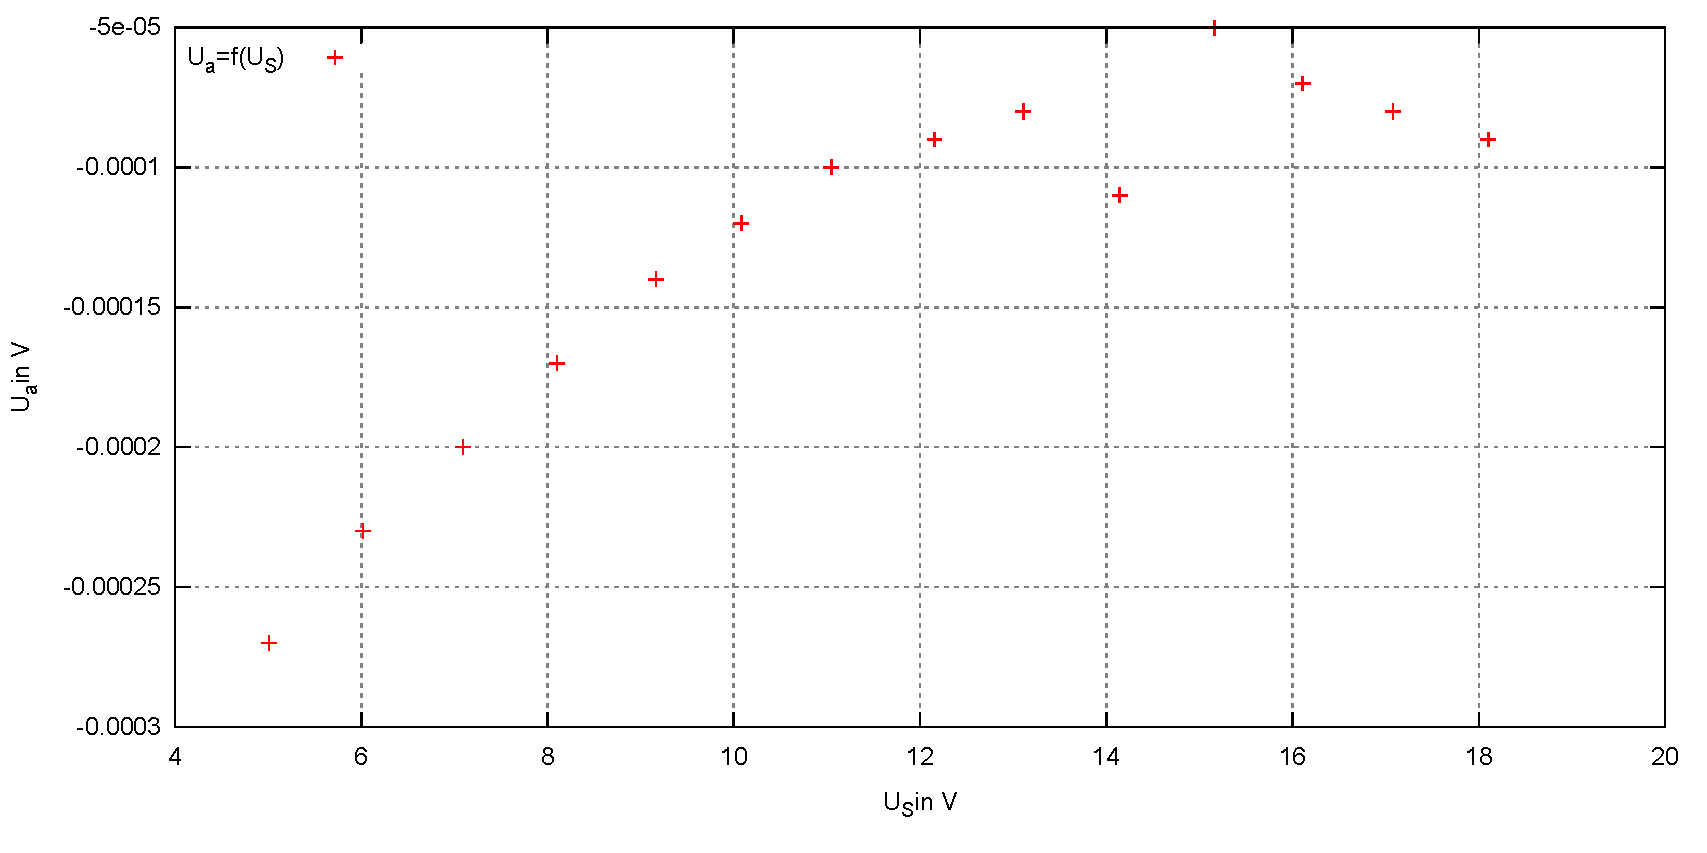
\includegraphics[width=\textwidth]{aufg1.pdf}
\caption{Messwerte zur Versuchsaufgabe 1}\label{img:aufg1}
\end{figure}
Der Durchgriff ist $\frac{\Delta U\ix{a}}{\Delta U\ix{S}}\approx0,02958$ für den nahezu linearen Bereich zwischen $U\ix{S}\approx\unit[5]{V}$ und $U\ix{S}\approx\unit[11]{V}$.
\subsubsection{Versuchsaufgabe 2}
\begin{figure}[H]
\centering
\begin{subfigure}[b]{\textwidth}
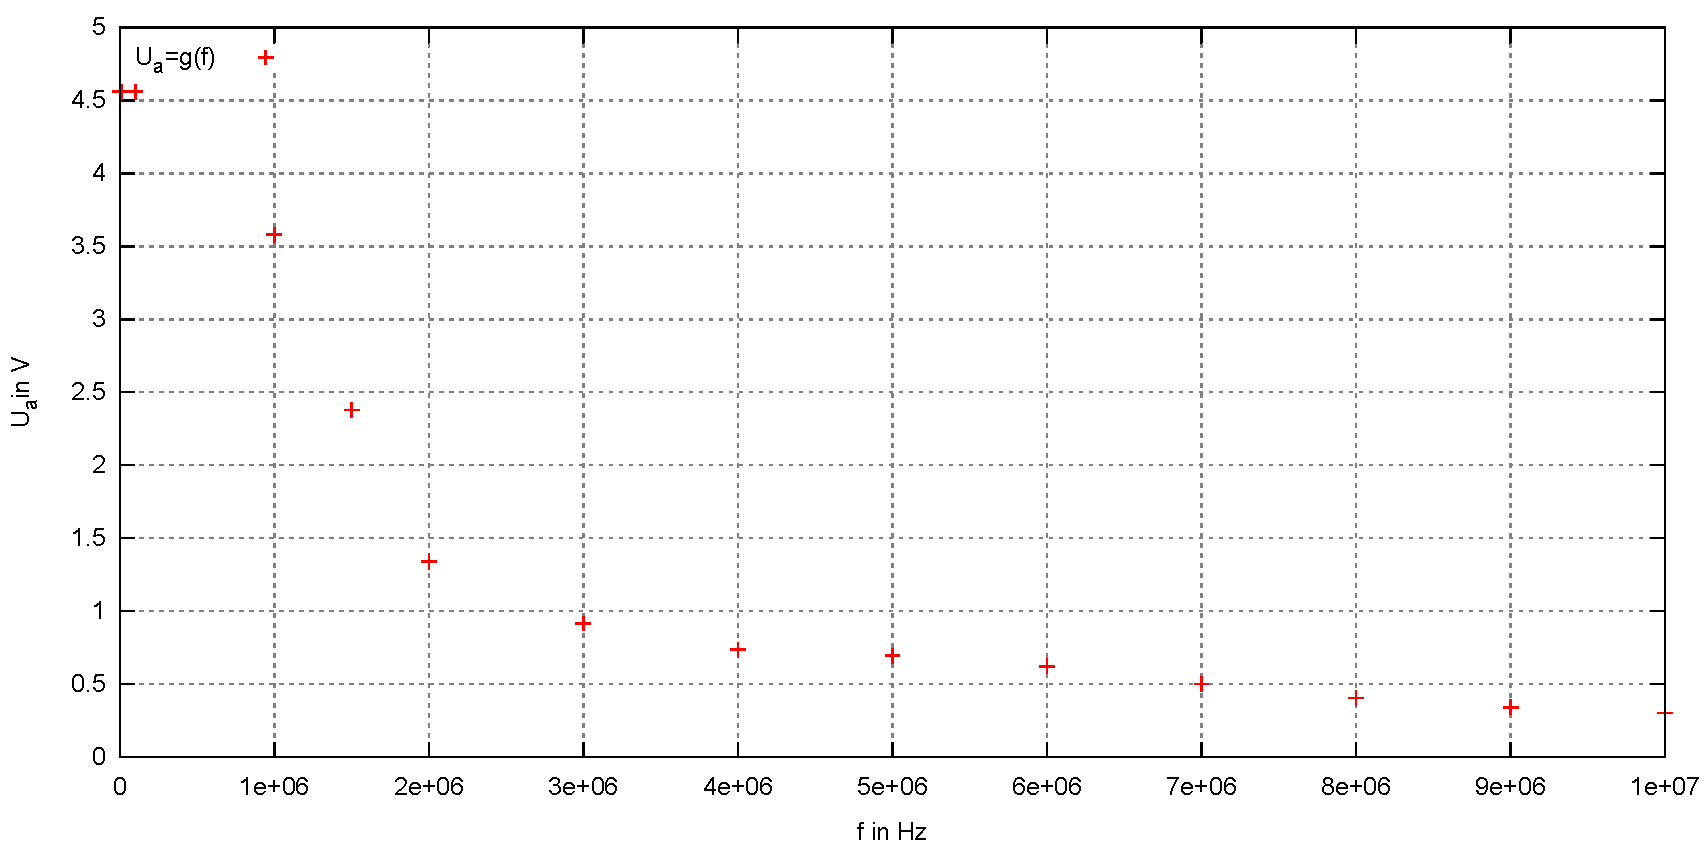
\includegraphics[width=\textwidth]{aufg2.pdf}
\caption{Ausgangsspannung $U\ix{a}$} \label{img:aufg2spannung}
\end{subfigure}
\begin{subfigure}[b]{\textwidth}
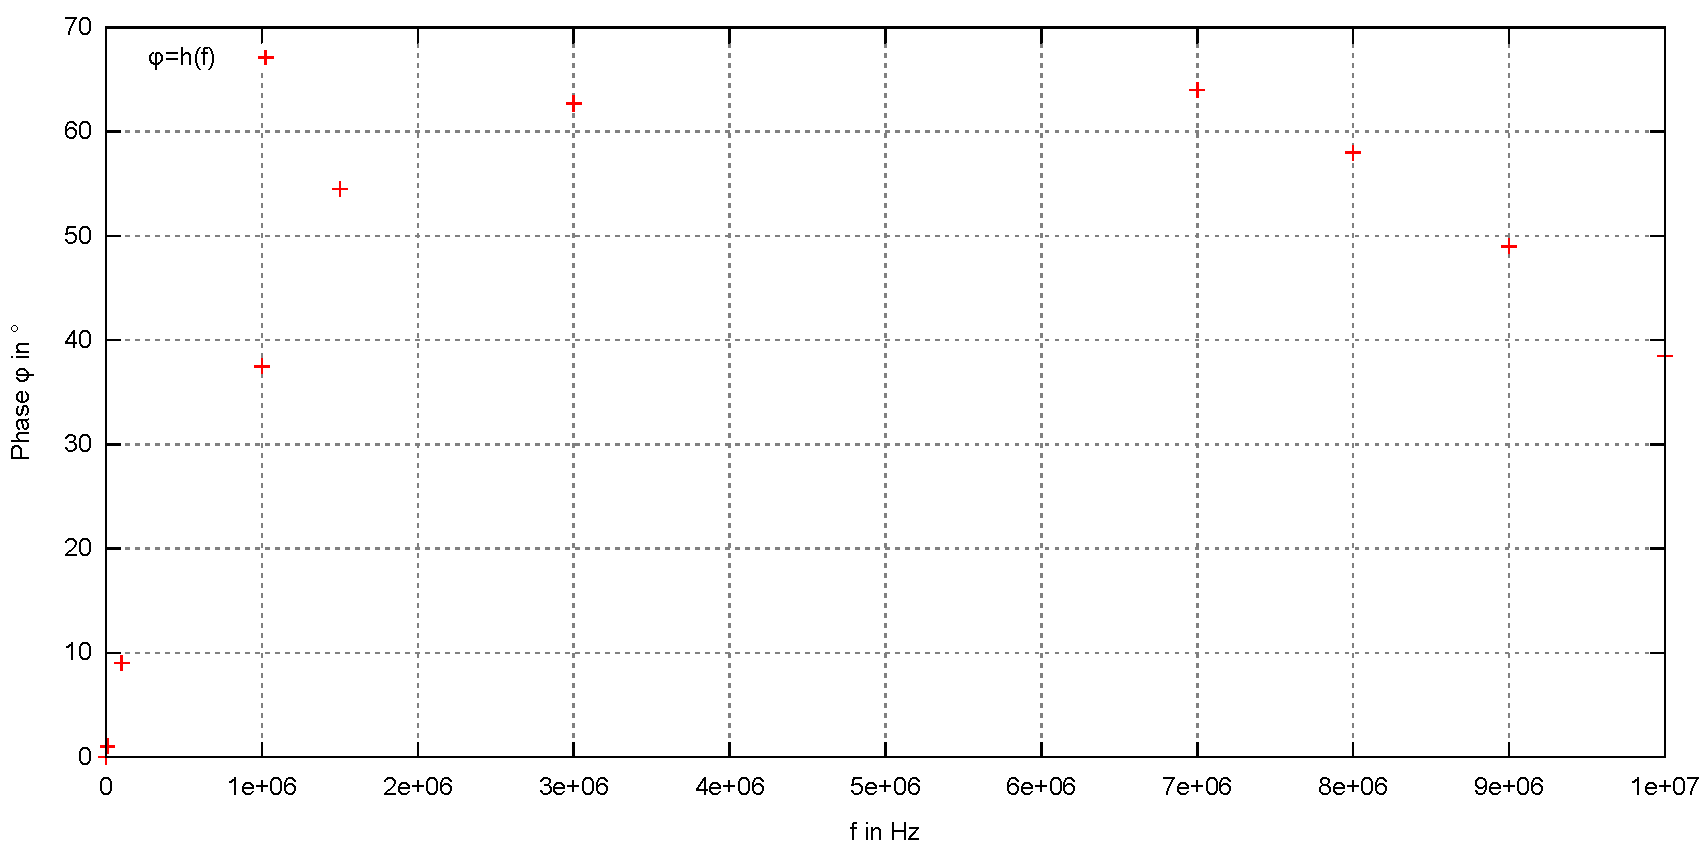
\includegraphics[width=\textwidth]{aufg22.pdf}
\caption{Phase $\varphi$} \label{img:aufg2phase}
\end{subfigure}
\end{figure}
\subsubsection{Versuchsaufgabe 3}
Die Messergebnisse zu dieser Aufgabe sind nicht verwertbar. Sie hatten in keiner Weise etwas mit den Erwartungen oder Erfahrungen zu OPVs gemeinsam. Beispielsweise lies sich eine Transitfrequenz von nur $f\ix{t}\approx\unit[10]{kHz}$, bei einer gleichzeitig betrachteten Grenzfrequenz von $f\ix{g}\approx\unit[700]{kHz}$, messen. Außerdem war das Rauschen so stark, dass quasi keine Oszillographie durchgeführt werden konnte.
\subsubsection{Versuchsaufgabe 4}
\begin{figure}[H]
\centering
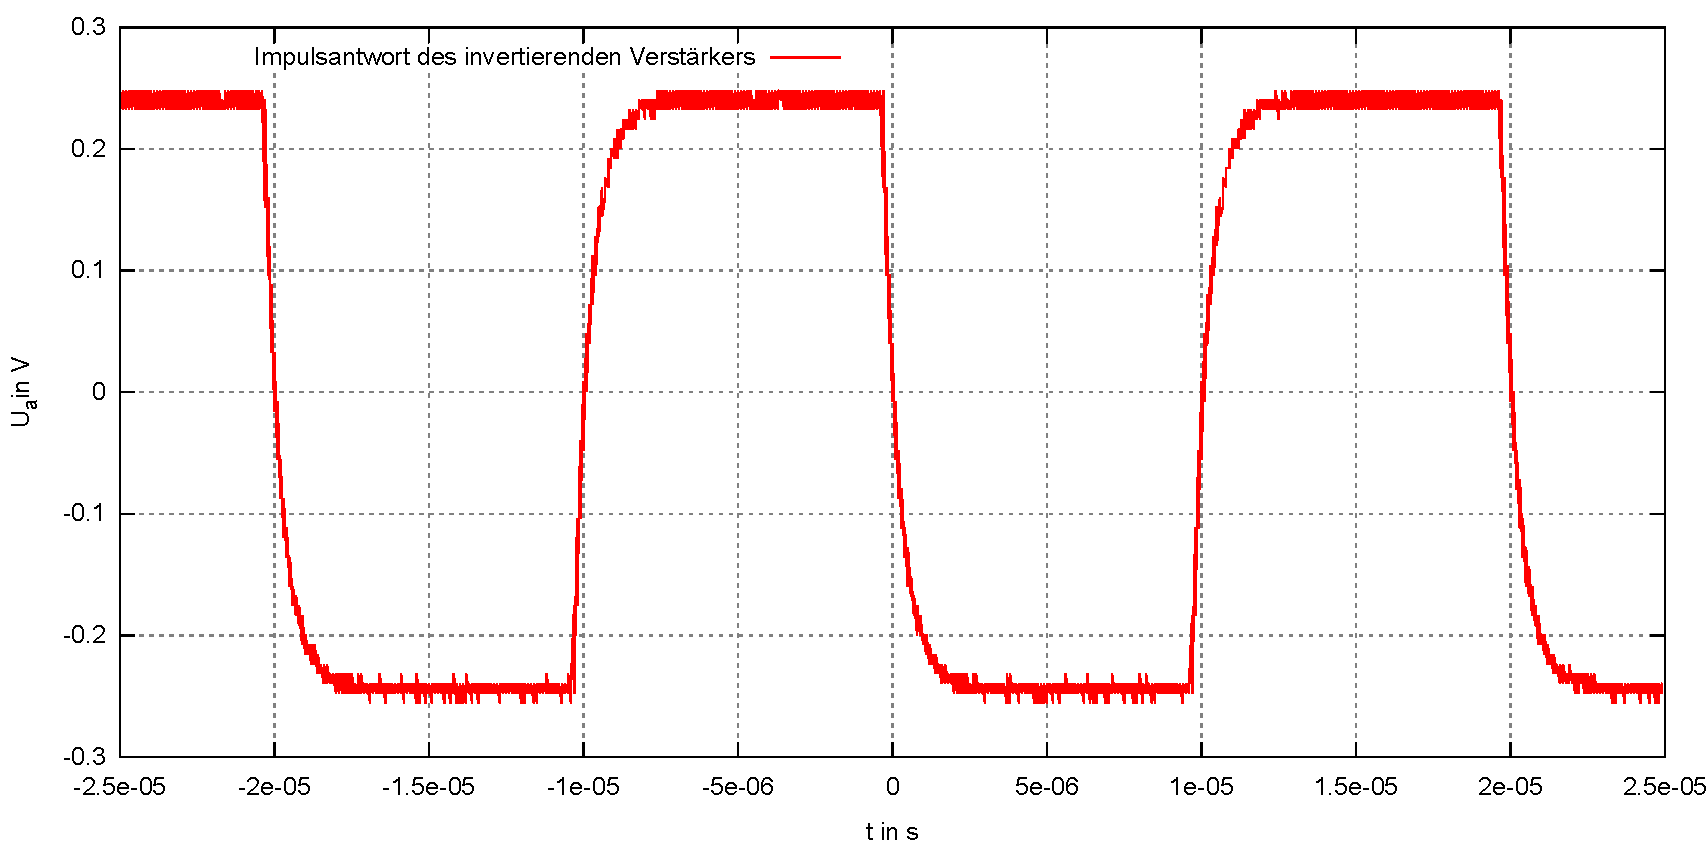
\includegraphics[width=\textwidth]{aufg4.pdf}
\caption{Diagramm zur slew rate $S\ix{r}$} \label{img:aufg4}
\end{figure}
Für die Vorderflanke ergibt sich die slew rate zu $S\ix{r;V}=\unit[1,29]{\frac{V}{\mu s}}$. Die slew rate der Rückflanke ist $S\ix{r;R}=\unit[0,9553]{\frac{V}{\mu s}}$. Die Großsignalbandbreite bei einer Spannungsamplitude $\hat{U}\ix{a}\approx\unit[260]{mV}$ ergibt sich somit zu $f\ix{GS}=\unit[792,173]{kHz}$.
\subsubsection{Versuchsaufgabe 6}
In einem Zeitintervall von $\Delta t=\unit[890]{ns}$ wuchs die Spannung um $\Delta U=\unit[26,2]{V}$. Damit ist die slew rate $S\ix{r}=\unit[29,43]{\frac{V}{\mu s}}$.
\subsection{Oszillogramme}
\subsubsection{Versuchsaufgabe 4}
\begin{figure}[H]
\centering
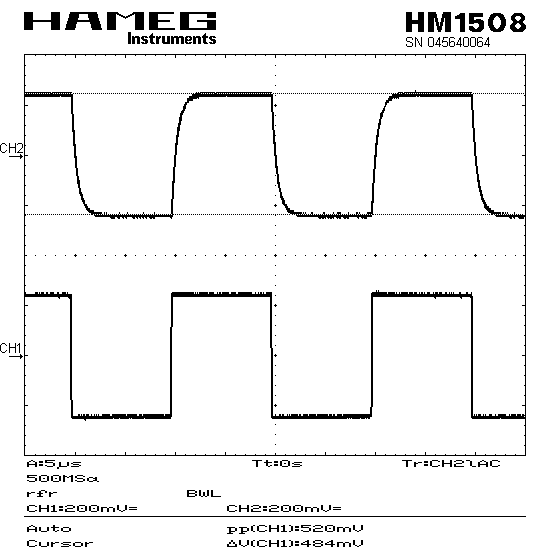
\includegraphics[width=0.5\textwidth]{aufg4oszillo.png}
\caption{Impulsantwort des invertierenden Verstärkers bei $f\approx\unit[50]{kHz}$ und $\hat{U}_0\approx\unit[0,5]{V}$} \label{img:oszillo}
\end{figure}
\subsubsection{Versuchsaufgabe 5}
\begin{figure}[H]
\centering
\begin{subfigure}[b]{0.48\textwidth}
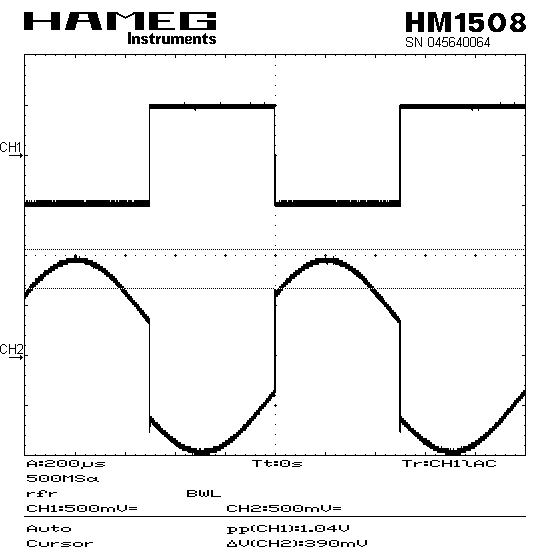
\includegraphics[width=\textwidth]{rechteck.png}
\caption{Vergleich Rechteck} 
\label{img:rechteck}
\end{subfigure}
\begin{subfigure}[b]{0.48\textwidth}
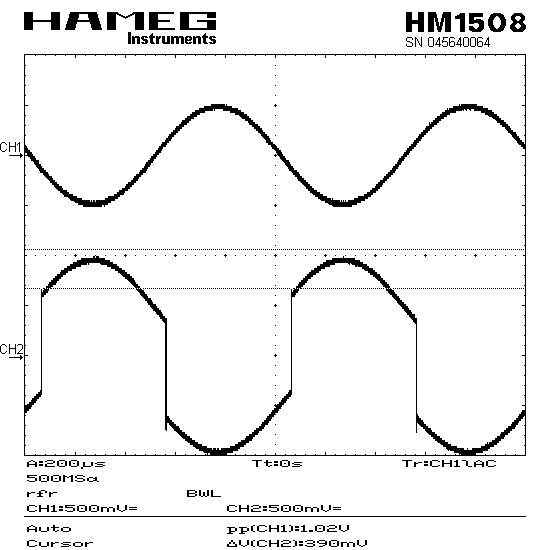
\includegraphics[width=\textwidth]{sinus.png}
\caption{Vergleich Sinus}
\label{img:sinus}
\end{subfigure}
\caption{Summation von Sinus- und Rechtecksignal bei Gewichtungsfaktor $t\ix{i}=-1$} \label{img:Summation}
\end{figure}
\end{document}